\documentclass[11pt]{article}

\usepackage[letterpaper,top=2cm,bottom=2cm,left=2cm,right=2cm,marginparwidth=1.75cm]{geometry}
\usepackage{hyperref}
\usepackage{biblatex}
\addbibresource{Bib.bib}
\usepackage{mathtools}
\DeclarePairedDelimiterXPP\BigOSI[2]%
  {\mathcal{O}}{(}{)}{}%
  {\SI{#1}{#2}}
\usepackage{xcolor}
\usepackage{empheq}
\usepackage[most]{tcolorbox}
\usepackage{amsmath}
\usepackage{amssymb}
\usepackage{mathrsfs}
\usepackage[utf8]{inputenc}
\usepackage{graphicx}
\usepackage{float}
\usepackage{parskip}
\usepackage{comment}
%\usepackage{mhchem}
 \usepackage{tabularx}
 \usepackage{titling}
 \usepackage{amsmath,environ}
 \usepackage[explicit]{titlesec}
\usepackage{fancyhdr}
\usepackage{braket}
\setlength{\droptitle}{3em} 

\title{Quantum Field Theory I}
\author{Thomas Brosnan}
\date{Notes taken in Professor Samson Shatashvili class, Michaelmas Term 2024}


\newtcbox{\mymath}[1][]{%
    nobeforeafter, math upper, tcbox raise base,
    enhanced, colframe=blue!30!black,
    colback=blue!30, boxrule=1pt,
    #1}
\tcbset{highlight math style={boxsep=2mm,,colback=blue!0!green!0!red!0!}}

\newenvironment{bux}{\empheq[box=\tcbhighmath]{align}}{\endempheq}
\newenvironment{bux*}{\empheq[box=\tcbhighmath]{align*}}{\endempheq}
\renewenvironment{flalign}{\empheq[box=\tcbhighmath]{align}}{\endempheq}
\renewenvironment{flalign*}{\empheq[box=\tcbhighmath]{align*}}{\endempheq}
\renewenvironment{flalign*}{\empheq[box=\tcbhighmath]{align*}}{\endempheq}





\newcommand{\hsp}{\hspace{8pt}}

\newcommand*{\sectionFont}{%
  \LARGE\bfseries
}

\newenvironment{eq}{\begin{equation}}{\end{equation}}
    
\numberwithin{equation}{section}

\makeatletter
\let\Title\@title % Copy the title to a new command
\makeatother

%change this RGB value to change the section background colour 
\definecolor{mycolor1}{RGB}{125, 187, 242}
\colorlet{SectionColour}{mycolor1}
%subsection background colour 
\definecolor{mycolor2}{gray}{0.8}
\colorlet{subSectionColour}{mycolor2}
%subsubsection background colour 
\definecolor{mycolor3}{RGB}{255,255,255}
\colorlet{subsubSectionColour}{mycolor3}


\begin{document}

\maketitle

\newpage
\topskip0pt
\vspace*{\fill}
\begin{center}
\Large
    "We will work in "God-given" units, where $\hbar = 1 = c$" 

    -Peskin \& Schroeder  
\end{center}
\vspace*{\fill} 
\newpage 
\tableofcontents
% For \section
 \titleformat{\section}[block]{\sectionFont}{}{0pt}{%
 \fcolorbox{black}{SectionColour}{\noindent\begin{minipage}{\dimexpr\textwidth-2\fboxsep-2\fboxrule\relax}\thesection  \hsp #1 {\strut} \end{minipage}}}
% For \subsection
 \titleformat{\subsection}[block]{\bfseries}{}{0pt}{%
 \fcolorbox{black}{subSectionColour}{\noindent\begin{minipage}{\dimexpr\textwidth-2\fboxsep-2\fboxrule\relax}\thesubsection  \hsp #1 {\strut} \end{minipage}}}
% For \section*
 \titleformat{name=\section, numberless}[block]{\sectionFont}{}{0pt}{%
 \fcolorbox{black}{SectionColour}{\noindent\begin{minipage}{\dimexpr\textwidth-2\fboxsep-2\fboxrule\relax} #1 {\strut} \end{minipage}}}
  % For \subsection*
 \titleformat{name=\subsection, numberless}[block]{\bfseries}{}{0pt}{%
 \fcolorbox{black}{subSectionColour}{\noindent\begin{minipage}{\dimexpr\textwidth-2\fboxsep-2\fboxrule\relax} #1 {\strut} \end{minipage}}}
 % For \subsubsection
 \titleformat{\subsubsection}[block]{\bfseries}{}{0pt}{%
 \fcolorbox{black}{subsubSectionColour}{\noindent\begin{minipage}{15cm}\thesubsubsection \hsp #1 {\strut} \end{minipage}}}
  % For \subsubsection*
 \titleformat{name=\subsubsection, numberless}[block]{\bfseries}{}{0pt}{%
 \fcolorbox{black}{subsubSectionColour}{\noindent\begin{minipage}{15cm} #1 {\strut} \end{minipage}}}
\newpage 
%header 
\pagestyle{fancy}
\fancyhf{} % Clear all header and footer fields
\fancyhead[L]{\Title}
\fancyhead[R]{\nouppercase{\leftmark}}
\fancyfoot[C]{-~\thepage~-}
\renewcommand{\headrulewidth}{1pt}





%starting document 
\normalsize
\newpage
\section{QFT trailer}
\begin{itemize}
  \item We wish to see if we can perform a calculation in quantum field theory, just by elementary means, i.e. via dimensional analysis ect.

  Consider the head on collision of an electron $e^{-}$ and $e^{+}$ that results in the production of a muon $\mu^{-}$ anti muon $\mu^{+}$ pair, shown below: 
\begin{figure}[H]
\centering
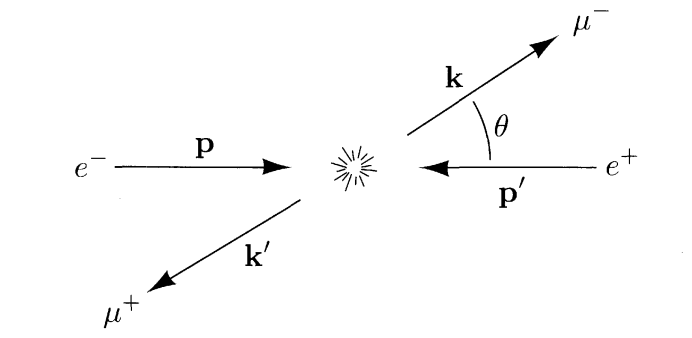
\includegraphics[width=0.6\textwidth]{trailer.png}
\caption{\label{trailer}\emph{electron positron annihilation}}
\end{figure}


\item The calculation we would like to perform is the differential cross section, that is the derivative of the cross section $\sigma$ with respect to the solid angle $\Omega$, $\frac{d \sigma}{d \Omega}$. This is a useful quantity as it is easily experimentally observed. In a particle collider, electrons and positrons are prepared in batches of length $l_A$ and $l_B$ and densities $\rho_A$ and $\rho_B$ respectively. When the two batches collide if the over lapping area of the head on collision is A, then the cross section is given by:
\end{itemize}
\begin{align*}
  \sigma = \frac{\text{Number of events}}{\rho_A\rho_B l_A l_B A}
\end{align*}

\begin{itemize}
  \item We now look at the dimensions of our quantities. Conveniently from our use of God given units, i.e. $\hbar =c =1$ we have that momentum, mass and energy have the same units as the energy mass equivalence becomes $E^2 = p^2 + m^2$. We also have from the Heisenberg's uncertainty principle that $\Delta p \Delta x \sim 1$. Thus the dimensions of mass and length are inversely related. 

  We can from this easily see that the dimensions of the quantity $[\rho_A\rho_B l_A l_B A]$ is $[m^2]$, which makes the dimensions of $\left[\frac{d\sigma}{d \Omega}\right] = \left[\frac{1}{m^2}\right]$ as angles are unitless. With this we can say that this quantity is also inversely proportional to the energy squared times some positive quantity that depends on the angle:


\begin{flalign}
  \frac{d\sigma}{d \Omega} \propto \frac{1}{E^2}|\mathcal{M}(\theta)|^2
\end{flalign}
Here $\mathcal{M}$ is a dimensionless quantity, that is essentially the quantum mechanical amplitude for the process to occur. It does not depend on the energy $E$, as we are considering the limit where $E >> m_e,m_{\mu}$. This means we are unable to construct any dimensionless quantity like $E/m_e$ or $E/m_{\mu}$ as we have set $m_e/E = 0 = m_{\mu}/e$. Note that we could not take this limit and them $\mathcal{M}$ would depend on $E$, but it is simpler to consider the high energy limit. 
\end{itemize}
\begin{itemize}
  \item If we recall from Quantum mechanics, in perturbation theory we had that at first order the transition amplitude is related to the initial and final states along with the interaction Hamiltonian $H_i$, so:

\begin{equation}
  \mathcal{M} \sim \bra{\text{final state}} H_I \ket{\text{initial state}}
\end{equation}
But we know physically that the electrons do not interact with the muons, Instead what we know happens is that the electrons annihilate to form photons which in turn form the muons. This then means that $\bra{\text{final state}} H_I \ket{\text{initial state}} = 0 $ and instead we have that:

\begin{align}
  \mathcal{M} \sim 
\end{align}
\end{itemize}

\end{document}
